%
% CSC 544 Final Project
% 
% @author Benjamin Dicken
% @author Rachel Baumann
%


\documentclass[a4paper, 12pt]{article}
\usepackage{comment} % enables the use of multi-line comments (\ifx \fi) 
\usepackage{fullpage} % changes the margin

\usepackage[english]{babel}
\usepackage[utf8x]{inputenc}
\usepackage{amsmath}
\usepackage{graphicx}
\usepackage{mathtools}
\usepackage{hyperref}
\usepackage{latexsym}
\usepackage{amssymb}
\usepackage{amsfonts}
\usepackage{amstext}
\usepackage{multicol}
\usepackage{amsxtra} 
\usepackage[margin=0.7in]{geometry}
\usepackage{algorithm2e}
\usepackage{framed}
\usepackage{booktabs}
\usepackage{color}


\title{CSc 544 Final Project}
\author{Benjamin Dicken and Rachel Baumann}

\begin{document}
\maketitle

\section*{The Dataset}

%Description of the data set we're using goes here...
%
%colors.csv
%pieces.csv
%sets.csv
%set\_pieces.csv
%
%images:
%parts
%sets

We are using a dataset from \href{http://rebrickable.com/}{Rebrickable.com} on the inventories of every official LEGO set up to 2015. This dataset includes 9,992 lego sets, 21,089 unique pieces in 130 colors, with a total of 479,751 relations between the sets and pieces. This dataset also includes images of 9,457 of the sets and most of the pieces. All data for the sets, pieces, colors, and maps between the pieces and sets are stored in csv files and the images are jpeg files. We have the following information in the fours csv files:

\begin{enumerate}

\item {\bf Sets:} Includes an ID for each set, the year a set was released, the total number of pieces in a set, and a category and brief description for each set.

\item {\bf Pieces:} Includes an ID, category and brief description for each piece.

\item {\bf Set Pieces:} Includes a set and piece ID, the number of times the piece is used in the set, the color of the piece in the set, and whether the piece is a normal or spare piece (called the piece type where 1 is normal and 2 is spare).


\item {\bf Colors:} Includes an ID and a brief description for each color.

\end{enumerate}

Downloading the data was a relatively straightforward process. All of the information for sets, pieces, colors, and the mapping between sets and pieces came as well-organized csv files packed into a single zip file. All we had to do was extract the data from the zip. The piece images also came bundled in zip files. Getting the images for the sets was a little trickier. \texttt{rebrickable.com} does not distribute those images in an easy-to-download format. To get the images, we wrote a simple web-scraper (in \texttt{bash}) which crawled \texttt{rebrickable.com} for all the images. We discovered that most of the data was in-tact and well-organized, so it needed very little cleaning. One issue we ran into was a few missing piece and set images, but this was minor. Another issue we ran into later was in order to incorporated the set ID and piece IDs into the HTML element ID names we had to replace any periods in the IDs with underscores since periods aren't allowed in HTML ID names. We fixed most of these issures as we read in the data.

\section*{The Visualization}

Our visualization consists of a three window linked view with a search bar and drop down menu on top. The window on the left shows an overview of the LEGO sets from a specified category plotted based on how similar their set descriptions are to one another The middle window shows a collection of six scatterplots with all sets plotted on each scatterplot based on two varying attributes. Finally, the last window shows the set image and specific set information in a table for a selected set. We'll refer to these windows as the t-SNE plot, the scatterplots, and the table plot in that respective order. All three windows and the search bar are connected by the same data and update if any other is used by the user.

\begin{figure}[h!]
\centering
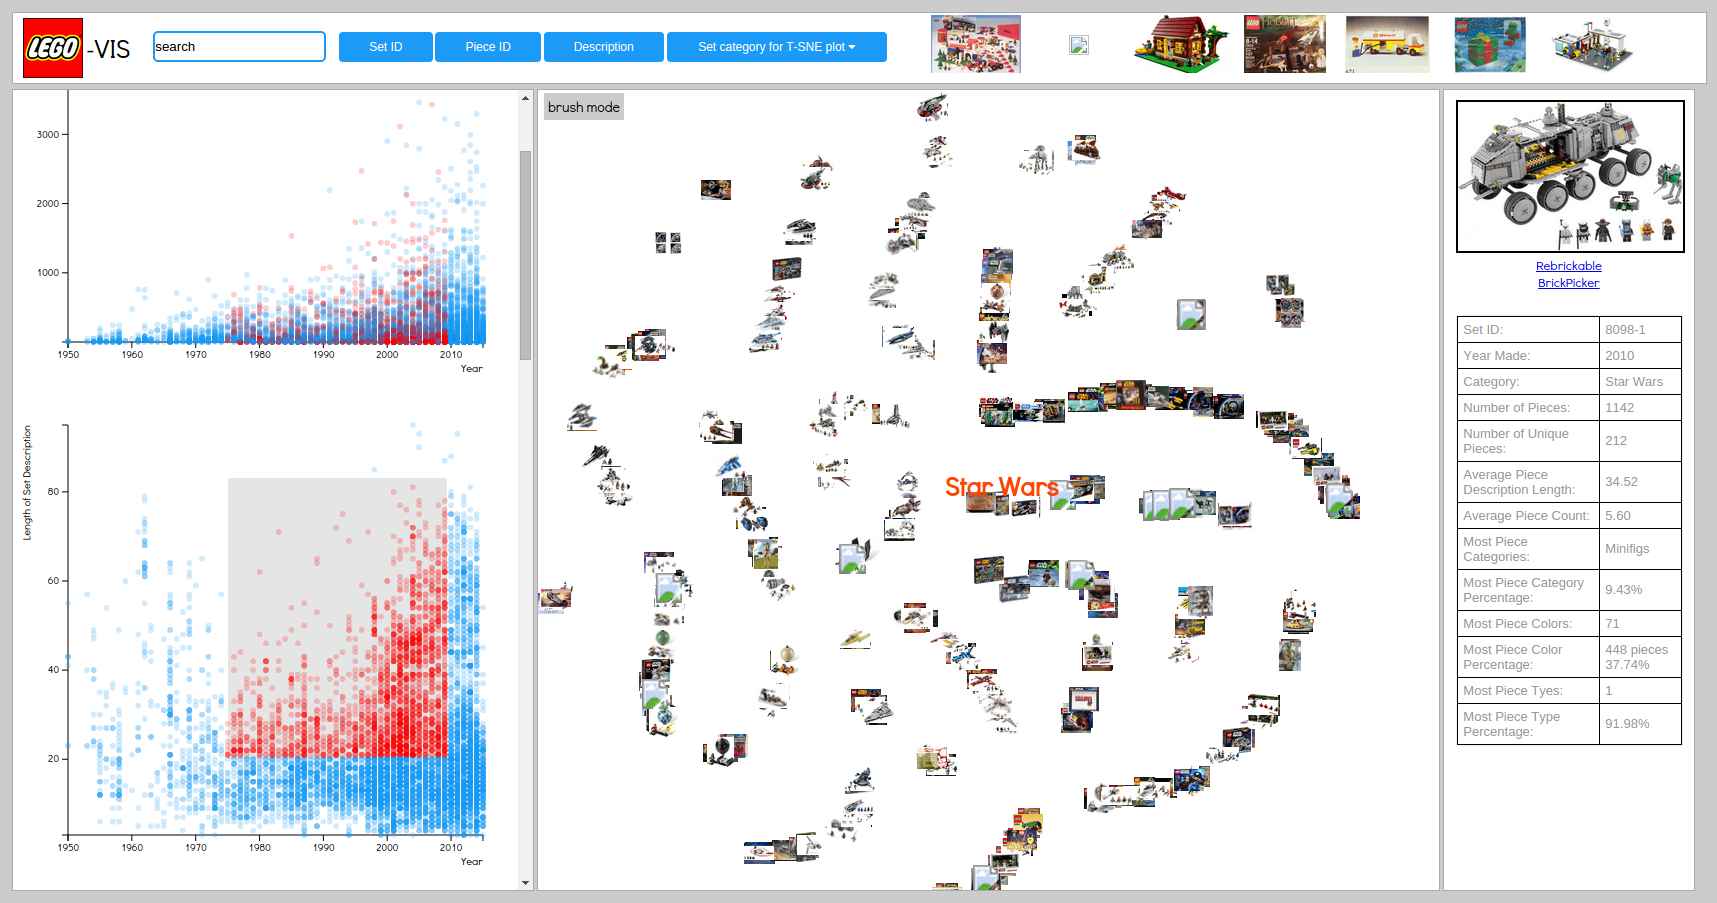
\includegraphics[width=1.0\textwidth]{img/lego-vis-screenshot.png}
\caption{UI for the LEGO visualization.}

\end{figure}

\subsection*{Overview}

To provide the user with a general overview of the data we show 6 scatterplots in which all sets have been plotted. We choose scatterplots for two varying attributes of  each set to one, not overwhelm the user with information but give them a few for the many dimensions of the data and two, because scatterplots are easy for users to read and gather information from acurately. The following six scatterplots where choosen from many scatterplots we experimented with because we either thought the relation was quite relevant or that the visual relation looked interesting. \\

The first scatterplots shows the relation between the number of pieces in a set and the time the set was created in which we observed an almost exponential increasing in the number of pieces being used in a set over the 65 years we have data for LEGO sets. The next shows the relation between the year the set was created and the length of the set description followed by the third plot showing a perhaps unintuitive relation between the length of the set description and the number of pieces in a set. What we found was an inverse relationship between the two largely due to the collection of minifigures which have few pieces but detailed descriptions. The next two plots shows the number of unique pieces in a set plotted agains the year the set was created  and  then agianst the total number of pieces in the set. The fourth scatterplot is very similar in nature to that of the first and the fifth shows a very distinctive linear trend. Lastly, the sixth scatterplot shows the relation between the type percentage of the pieces and the year the set was created. \\

In each scatterplot we plotted a set as a circle of radius 3 pixels  due to having almost 10,000 points on each plot but still wanting to allow the user the ability to click the points. We also gave each point an  opacity of 0.2 to show the density of each clustering of points on the scatterplots. The plots we kept as simple as possible so as not to add or take aways from the data itself. We made a compromize here to not show a global view of the t-SNE plot for all 10,000 sets in order to increase the speed of the visualization as a whole. In the end we settled on allowing the user to first filter the sets by category before showing the t-SNE plot.

\subsection*{Filter and Zooming}

In our visualization we provide filtering and zooming in three areas: the t-SNE plot by selction, the scatterplots with brushing, and the seach bar with searching based on a key word or partial set or piece ID. Here was where we had to make the most compromizes in terms of the speed of our visualization and the users freedom in filtering and zooming in on the data. Speed won almost every time.\\

On the t-SNE plot we allow the user to filter the sets based on the set category using a dropdown menu. Once a category is selected the collection of sets from this category is then plotted on a 2D plot using the t-SNE algorithm. The t-SNE algorithm works as follows. 
For the vector of similiarties, which t-SNE requires to be created for each node on the graph, we created a custom similarity function. 
First, we compute a set of tokens (along with a count representing number of occurrences) for each lego-set category. The set of tokesn for a category is generated by grabbing all of the tokens from the set description for each set in the category.
Next we computed a set of description tokens for each lego set, using all the tokens found in the set's description and the description of all it's pieces. For LEGO category, we add a number to the similarity vector. For a given category, we iterate through all of the lego sets tokens and count how many appear in the categorie's token list. The sum is the number we add to the vector. Each set, along with it's computed similarity vector, is passed along to the t-SNE algorithm and visualized. The user can then zoom in on this plot or brush. When brushing, the brushed elements are highlighted in the scatterplots. \\

Another way the user can filter the data is using brushing on anyone of the scatterplots. The points in the brush are highlighted red as are all points corresponding to these sets on all other scatterplots. With 10,000 points brushing can be slow so we improved the brush speed by only updating the points in the brush once the brush has been released by the user and by not changing the opacity of the points outside of the brush. It's still a bit slow but not nearly as slow as it was when it was updating as the user moves the brush. Again, because of the density of some of the clustering of points on the scatterplots we kept the points in the brush all at 0.2 opacity. We placed the brush first on all scatterplots to allow the user the ability to select points on the plots in or out of brushing. However, in areas of high density with no visible bacground the user won't be able to begin brushing.\\

The last way we allow the user to filter the data on the scatterplots is through the search bar. Here the user can search by a partial set or piece ID or with a brief desription. Then all sets having the same substring entered by the user in either it's set ID, piece ID, or set description will be highlighted on all plots in yellow with opacity 1 and brought to the front of the plot. Here we compromised on speed by only allowing the user the ablility to either search or brush but not both at once and the user must specify whether to seach by set ID, piece ID or by description.

\subsection*{Details on Demand}

By selecting a single point on any of the scatterplots or on the t-SNE plot, all points corresponding to this set are highlighted and we show an image of it (if available) plus a table of information for the selected set given beneath it. In addition, we provide links to view the selected set on \texttt{rebrickable.com} and \texttt{brickpicker.com}. \\

When a user searches by a specific Set ID, Piece ID, or if the search only had one result then the point is still highlighed as described in filtering but we also bring up the set image and table of set information in the table. \\

At the top of the page (in the menu bar) there are changing images of ramdom LEGO sets. If one is clicked on, all points corresponding to that set will be highlighted on all scatterplots and the image and table of set information will appear in the table. \\

\subsection*{Source Code}

All the soruce code for this project is available at \texttt{https://github.com/bddicken/lego-vis}.


\end{document}

